\documentclass[runningheads]{llncs}
%
\usepackage{todonotes}
\usepackage{graphicx}
\usepackage[
    n,
    advantage,
    operators,
    sets,
    adversary,
    landau,
    probability,
    notions,
    logic,
    ff,
    mm,
    primitives,
    events,
    complexity,
    asymptotics,
    keys]{cryptocode}

\begin{document}

\title{Website and Application Data Fingerprinting \\ Past, Present, and Future}
\author{Christopher A. Wood}
\authorrunning{C. Wood}
% \institute{Wat, USA \and
% Springer Heidelberg, Tiergartenstr. 17, 69121 Heidelberg, Germany
% \email{lncs@springer.com}\\
% \url{http://www.springer.com/gp/computer-science/lncs} \and
% ABC Institute, Rupert-Karls-University Heidelberg, Heidelberg, Germany\\
% \email{\{abc,lncs\}@uni-heidelberg.de}}

\maketitle
\begin{abstract}
TLS 1.3 is a substantial update to a fundamental security protocol used on the Internet. 
Beyond notable performance improvements, the new design yields security properties desired
for modern network communication, including: forward-secure session key secrecy, downgrade
protection, key compromise impersonation resistance, and protection of endpoint identities. 
Also, more of the protocol messages are encrypted end-to-end, thereby offering improved
privacy to clients and servers. As a greenfield protocol, IETF QUIC goes further by encrypting
as much of the protocol messages as possible without compromising on desired transport
properties, such as connection identifier-based mobility. Combined, these two protocols 
are set to protect a significant amount of Internet data. However, significant metadata leaks still exist,
including: plaintext TLS SNI and application-specific extensions (ALPN) and DNS queries.
The IETF is well on its way to protecting this metadata with protocols such as DNS-over-TLS 
and DNS-over-HTTPS, and work-in-progress towards encrypting the SNI. However, we argue that
much more work is needed to protect metadata, especially in the context of web traffic. 
In this paper, we survey Website Fingerprinting attacks, which are a class of attacks that
use machine learning techniques to attack web privacy, and highlight metadata leaks used
by said attacks. We also survey proposed mitigations for such leakage and discuss their 
applicability to IETF protocols such as TLS, QUIC, and HTTP. We endeavor to show that
Website Fingerprinting attacks are a serious problem that affect all Internet users, 
and we pose open problems and directions for future research in this area.

\keywords{IETF \and TLS \and QUIC \and Pervasive Monitoring \and Metadata Protection}
\end{abstract}

\section{Introduction}
Internet protocols such as TLS 1.3 \cite{rfc8446} and QUIC \cite{ietf-quic-transport-16} 
bring substantial improvements to end-users. 
The IETF engineered these with security and privacy in mind by encrypting
more protocol messages using modern cryptographic primitives and algorithms, and engineering
against flaws found in previous protocols, yielding several desirable security
properties, including: forward-secure session key secrecy, downgrade protection, key 
compromise impersonation resistance, and protection of endpoint identities. 
Combined, these two protocols are set to protect a significant amount of Internet data. 
However, significant metadata leaks still exist for users of these protocols. Examples include
plaintext TLS SNI and application-specific extensions (ALPN) and DNS queries. This information
can be used by a passive attacker to learn information about the contents of an otherwise
encrypted network connection. In the context of Tor, a popular low-latency anonymity
network, a common class of attacks that use metadata for such inference is called
Website Fingerprinting (WF). These attacks use machine learning techniques built with
features extracted from metadata such as traffic patterns to attack web (browsing) privacy.
Miller et al. \cite{miller2014know} show how these attacks can be applied to web browsing
traffic protected with HTTPS to reveal private information about users.
Fingerprinting attacks using encrypted traffic analysis are also applicable to encrypted
media streams, such as Netflix videos. (See work from Reed et al. \cite{reed2017identifying} 
Stikkelorum \cite{stikkelorum2017know}, and Schuster et al. \cite{schuster2017beauty} 
for examples of these attacks.)

The IETF is well on its way to protecting this metadata with protocols such as DNS-over-TLS 
and DNS-over-HTTPS \cite{rfc8484}, and work-in-progress towards encrypting 
the SNI extension \cite{ietf-tls-esni-02}. However, we argue 
that much more work is needed to protect metadata, especially in the context of web traffic. 
In this paper, we describe WF attacks in the context of IETF protocols
such as TLS and QUIC. We survey WF attacks and highlight metadata features used to conduct
said attacks. We also describe proposed mitigations for these attacks and discuss their
applicability to IETF protocols. We conclude with a discussion of open problems and directions
for future research and advocate for more work in this area. 

% http://delivery.acm.org/10.1145/2940000/2939929/p61-alan.pdf?ip=98.234.75.172&id=2939929&acc=CHORUS&key=4D4702B0C3E38B35%2E4D4702B0C3E38B35%2E4D4702B0C3E38B35%2E6D218144511F3437&__acm__=1542991706_beefa03762b98f822bd5969b8cd4fbdb
% https://ieeexplore.ieee.org/abstract/document/7448393/

\section{Background}
In this section we review how most secure Internet connections are made today. We omit custom 
configurations such as those using VPNs and proxies since they do not represent the common case
for most Internet users. Figure \ref{fig:connections-then} shows the sequence of events that 
normally occur when a web client, e.g., browser, {\tt curl}, etc., needs to connect to a website 
and obtain a resource. First an unencrypted DNS query is sent to an untrusted DNS recursive 
resolver to resolve a name to an IP address. Upon receipt, clients then open a TCP and TLS 
connection to the destination address. During this stage, metadata such as the TLS SNI and ALPN
values are sent in cleartext. The SNI is used to denote the destination application or endpoint
to which clients want to connect. Servers use this for several purposes, including selecting
an appropriate certificate (one with the SNI name in the SubjectAlternativeName list) or
routing to a different backend terminator. ALPN values are used to negotiate which application-layer
protocol will be used on top of the TLS connection. Common values include "http/1.1", "h2", and 
(soon) "h3". Upon connection, clients then send HTTP messages to obtain the desired resource. 

\begin{figure}
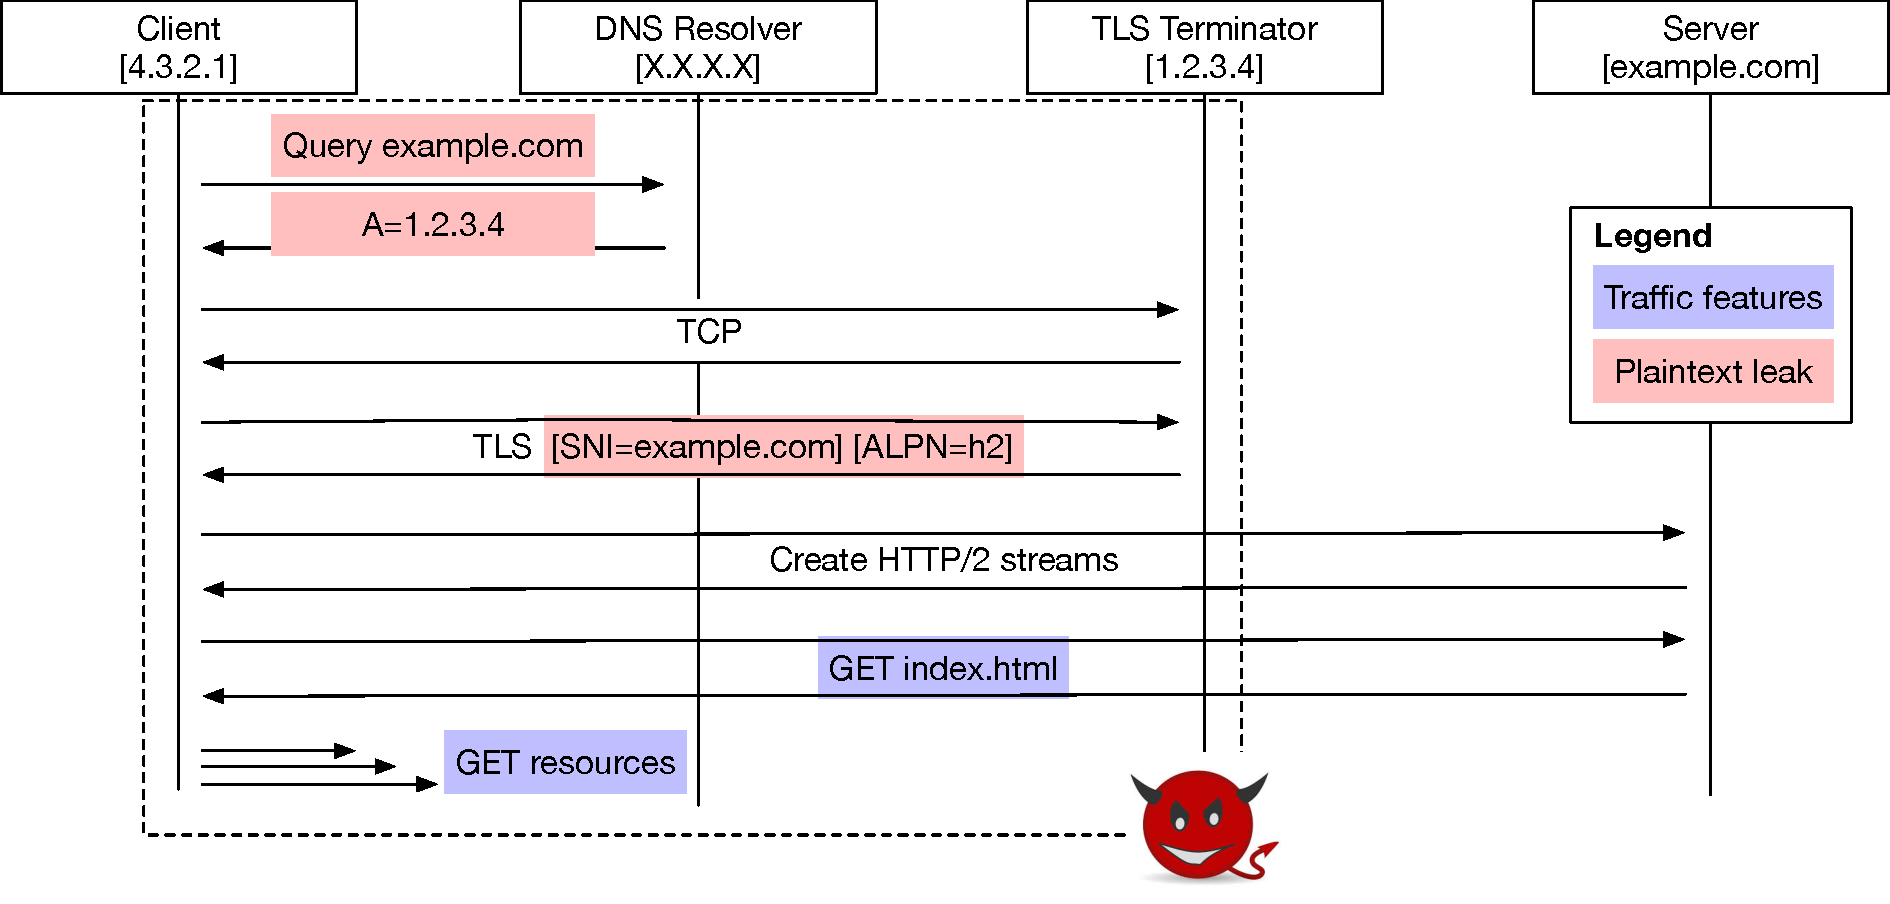
\includegraphics[scale=0.35]{figures/connection_flow}
\caption{Connections without Secure DNS or Encrypted SNI}
\label{fig:connections-then}
\end{figure}

Connections look different (on the wire) with TLS 1.3, encrypted DNS via DNS-over-TLS or
DNS-over-HTTPS, and encrypted SNI. Figure \ref{fig:connections-now} shows this variant.
DNS queries are encrypted to a (trusted) recursive resolver and TLS metadata such as SNI
are encrypted in transit to the terminator. Despite the reduction in cleartext metadata
sent over the wire, there still remains several sources of information that an adversary
may use for malicous purpuses, including: size and timing of DNS queries and responses, 
size and timing or application traffic, and connection attempts induced while loading a 
web resource, e.g., Javascript files. So while technologies such as Encrypted SNI, DoT,
and DoH help protect some metadata, they are not complete solutions to the larger problem.
In the following section, we discuss this overarching problem in detail.

\begin{figure}
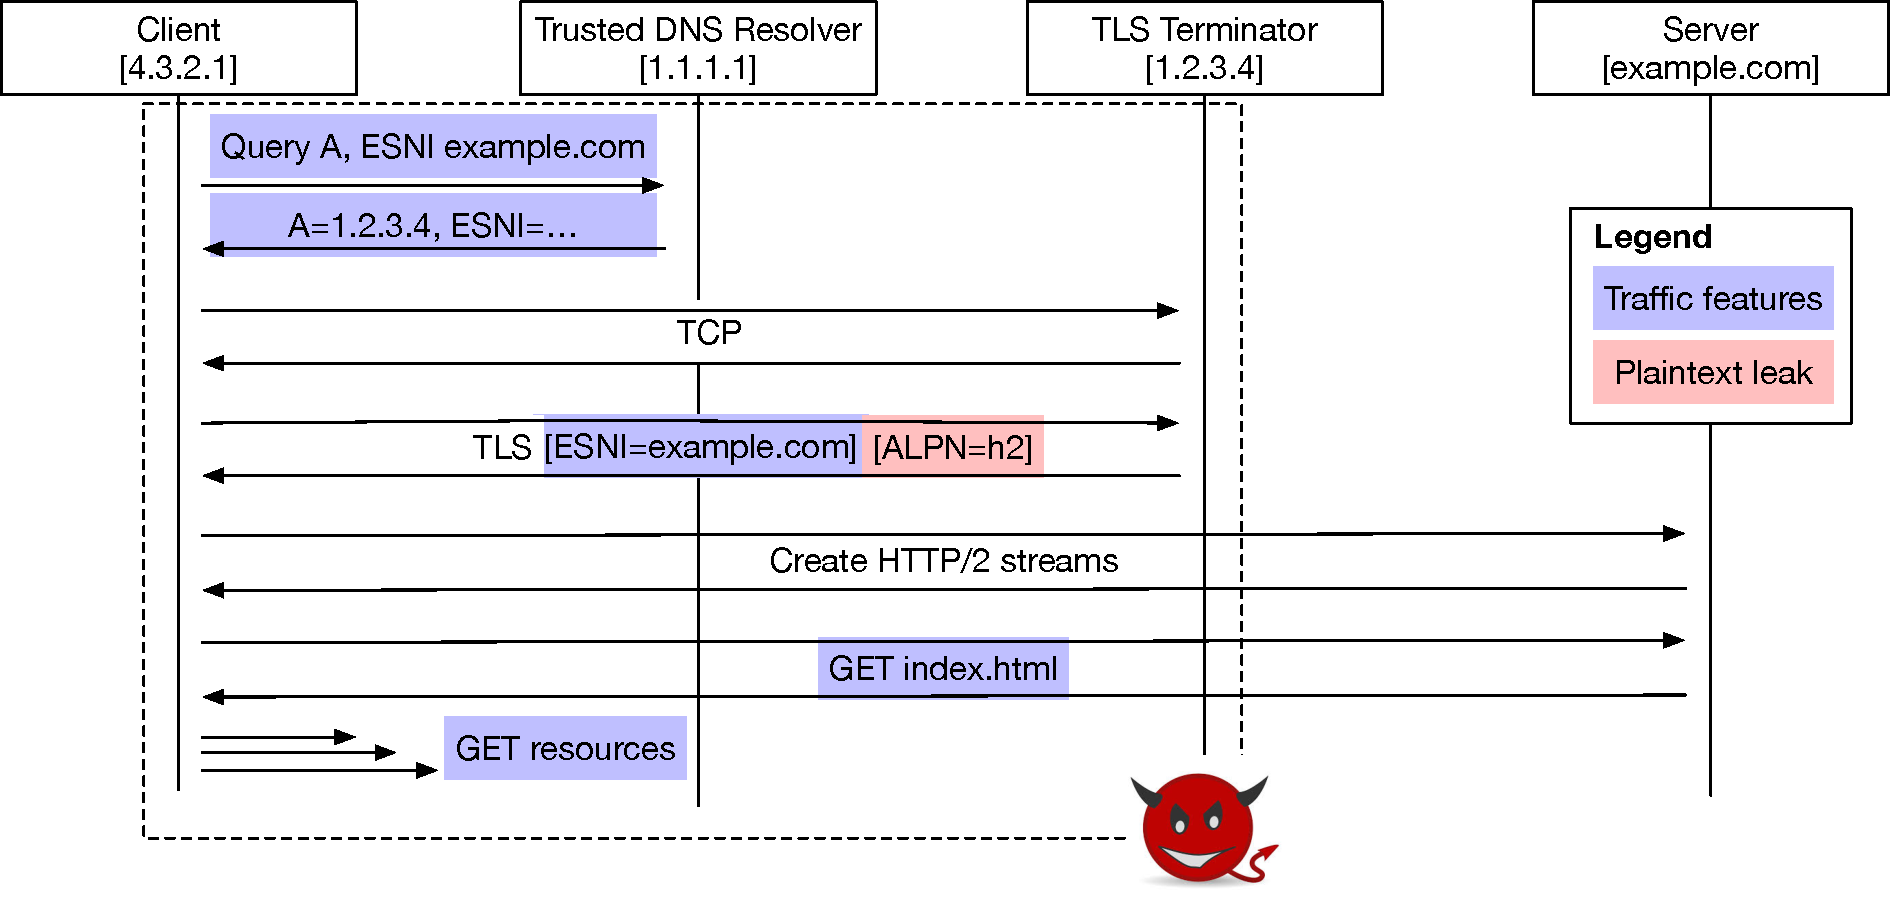
\includegraphics[scale=0.35]{figures/connection_flow_now}
\caption{Connections with Secure DNS and Encrypted SNI}
\label{fig:connections-now}
\end{figure}

%\todo[inline]{Discuss contents of page -- dynamic vs static}

% https://uwspace.uwaterloo.ca/bitstream/handle/10012/10123/Wang_Tao.pdf?sequence=3&isAllowed=y
\section{Website Fingerprinting}
Website Fingerprinting (WF) is a class of attacks that exploit metadata leakage to attack
end-user privacy on the Internet. There are two types of models to analyze these attacks:
open- and closed-world. The open world model assumes \adv\ wishes to learn whenever a victim
client visits one of a select number of \emph{monitored pages} \cite{wang2016website}. Adversaries train 
classifiers in this model using monitored and non-monitored websites of their choosing. By
defintion, \adv\ cannot train using client-chosen pages. Clients then visit pages at will
and \adv\ attempts to learn whenever a monitored page is visited, if any are at all. The closed
world model assumes clients only visit pages monitored by \adv\ and is thus a substantially
reduced threat model and not applicable to real-world scenarios.\footnote{\adv\ would need to
monitor \emph{every} possible page of interest to each client, which is impractical.}

\adv\ is assumed to be a passive and local attacker. Local means that \adv\ can associated 
traffic with a given client. Examples include proxies to which clients directly connect. 
Passive means that \adv\ can only view traffic in transit. It cannot add, drop, or otherwise
modify packets between the victim client and server(s). Use of reliable and encrypted transport
protocols such as TLS limit on-path attackers to eavesdropping on encrypted packets. (In
QUIC, however, reordering packets is possible.)

Traffic features used for classification include properties such as packet size, timing, 
direction, interarrival times, and burstiness, among many others \cite{wang2016website}. Normally, features
are restricted to those which are extractable as a passive eavesdropper, and not those which 
are viewable by modifying client or server behavior. Specifically, this means that
attacks such as CRIME \cite{} and TIME \cite{}, which rely on an attacker abusing TLS-layer compression
to leak contents of an encrypted connection, are out of scope. 

\subsection{Attacks}
WF attacks date back to applications on SSL first inspired by Wagner and 
Schneier \cite{wagner1996analysis}, in which the authors observed that 
packet lengths reveal information about the underlying data. Subsequent attacks
carried out by Cheng et al. \cite{cheng1998traffic}, 
Sun et al. \cite{sun2002statistical}, and Hintz \cite{hintz2002fingerprinting}. 
These attacks assume \adv\ has knowledge of the target resource length(s), 
which is not always possible with techniques such as padding. Shmatikov and Wang \cite{shmatikov2006timing} 
presented a WF attack that exploits cross correlation of arrival packet counts in
one second time windows. Bissias et al. \cite{bissias2005privacy} extend this idea to inter-packet
times in one second windows. Liberatore and Levine \cite{liberatore2006inferring} proposed two WF attacks
using different classification techniques. The first of which relies on the Jaccard 
coefficient to measure the similarity between unique packet lengths and \emph{classes}
of unique packet lengths.\footnote{The authors assume packets which do not fill a MTU
represent packet trailers. Therefore, uniqueness is only accurate modulo the MTU. Efficacy
is therefore limited if endpoints pad packets to the MTU or another fixed length.}
More similar sequences share larger numbers of unique packet lengths. The second 
attack compares unique packet length frequencies to frequencies of unique packet length
classes using a Naive Bayes classifier with kernel density estimation. As in the first 
attack, more similar sequences have more frequent unique packet lengths in common. 
Herrmann et al. \cite{herrmann2009website} extended the work of Liberatore and Levine with a multinomial
Naive Bayes classifier modified computed using three input frequency transformations. 
(That is, during the classifier probability calculations, packet length frequencies are 
transformed using different techniques.) This classifier assumes each packet length is 
independent from the rest. Results yielded higher accuracy than that of Liberatore and Levine.

Lu et al. \cite{lu2010website} developed a classifier based on the Levenshtein distance between
ingress and egress packet lengths extracted from packet sequences. Distance is computed between
strings of ingress and egress packet lengths. The training packet sequence with the closest 
distance to the testing packet sequence is deemed the match. Panchenko et al. \cite{panchenko2011website} 
were the first to use a support vector machine (SVM) classifier trained with web domain-specific
features, such as HTML document sizes, as well as packet lengths. Dyer et al. \cite{dyer2012peek}
used a Naive Bayes classifier trained with a reduced set of features, including total
response transmission time, length of pcakets (in each direction), and burst lengths.\footnote{Wang 
\cite{wang2016website} notes that measuring burst lengths in Tor is difficult given the presence of
SENDME cells for flow control.} This approach did not yield any measurable improvements over
the SVM classifier from Panchenko et al. Cai et al. \cite{cai2012touching} extend the work of Lu et al.
by adding transpositions to the Levenshtein distance computation and normalizing the result to
a value in $[0,1]$, yielding what the authors refer to as the Optimal String Alignment Distance 
(OSAD). Before feature extraction, the authors round TCP packet lengths to the nearest multiple of
$600$B as an estimate of the number of Tor cells. 

Wang et al. \cite{wang2013improved} tuned the OASD-based attack to improve its accuracy. Specific changes
include use of Tor cells instead of TCP packets for packet and burst lengths, as well as heuristics
to remove SENDME cells (those not carrying application data) from flows to recover true
burst lengths. The authors also modified the distance computation by removing substitutions,
increasing the weight for egress packets, and varying the transposition cost across the packet
sequence (large weights at the beginning of a trace, and smaller weights near the end, where
variations are expected across repeated page loads.) Wang et al. also developed an alternate classifier
with lower accuracy yet superior performance (quadratic to linear time complexity). It works by 
minimizing the sum of two costs: sequence transpositions and sequence deletions or insertions. These 
two costs are computed separately, in contrast to the first approach which computes them simultaneously.

Wang et al. \cite{wang2014effective} also developed an attack using a $k$-Nearest Neighbors ($k$-NN) classifier,
which is a supervised machine learning algorithm, targeting the open world setting. The classifier
extracts a large number of features from packet sequences, including raw (ingress and egress)
packet counts, unique packet lengths, direction, burst lengths, and inter-packet times, among others.
(There are $4226$ features in total.) The $k$-NN distance metric is computed as the sum of weighted 
feature differences. 

Kota et al. \cite{abe2016fingerprinting} were the first to use Deep Learning (DL) methods based on Stacked 
Denoising Autoencoders for WF attacks. (Autoencoders reduce feature input dimensions when stacked.)
Kota et al. form input vectors from Tor cell directions ($+1$ or $-1$). They use no other features.
Using a (small) data set from Wang \cite{wang2016website}, the classifier achieves a $86\%$ true positive 
rate and $2\%$ false positive rate in the open world model. Rimmer et al. \cite{rimmer2018automated}
applied DL for automated feature generation and classifier construction. Trained with $2,500$ traces
per website, their system achieves $96.3\%$ accuracy in the open world model. Yan et al. \cite{yan2018feature}
studied manual high-information feature extraction from packet traces. They ``exhaustively'' examined different 
levels of features, including packet, burst, TCP, port, and IP address, summing to $35,683$ in total, and 
distilled them into a diverse set of uncorrelated features for eight different communication scenarios. 
Recently, Bhat et al. \cite{bhat2018var}, Oh et al. \cite{oh2017pfp}, and Sirinam et al. \cite{sirinam2018deep}
used Convolutional Neural Networks (CNNs) and Deep Neural Networks (DNNs) for WF attacks. Results from
Sirinam et al. show the best results -- $98\%$ on Tor without recent defenses (in Section \ref{sec:defenses}) -- 
while performing favorably when select defenses are used.

\subsection{Defenses} \label{sec:defenses}
WF defenses are deterministic or randomized algorithms that take as input application data or a packet sequences
and return modified application data or packet sequences. Viable defenses seek to minimize the transformation
cost and maximum (theoretical and perfect) attacker accuracy. Naive defenses such as sending a constant stream
of (possibly random) bytes between client and server may be effective though are clearly not viable from a cost
perspective. Relevant cost metrics include bandwidth overhead, added time or latency (and its impact on related
metrics such as page load time), and even CPU cost, though the latter is often ignored in favor of the former two.
Wang \cite{wang2016website} describe defenses as either \emph{limited} or \emph{general}. A limited defense is
one which only helps mitigate specific WF attacks by transforming packets in a way to obviate a particular 
(set of) feature(s) used by said attacks. In contrast, general defenses help mitigate a variety of attacks.

Many limited defenses have been proposed. We list prominent works below.
\begin{itemize}
\item Shmatikov and Wang \cite{shmatikov2006timing} developed adaptive padding which adds packets to mask 
inter-packet times. (This mechanism does not ever delay application data being sent, in contrast to other
padding mechanisms such as BuFLO; see below.) 
Juarez et al. \cite{juarez2016toward} also created a WF defense based on adaptive padding called WTF-PAD. 
This variant uses an application data and ``gap'' distribution to generate padding for delays. When
not sending application data, the gap distribution is used to generate fake sample sizes for transmission.
WTF-PAD can be run by a single endpoint, though it is assume that both client and server participate.
\item Wright et al. \cite{wright2009traffic} developed traffic morphing, which pads packets in such a way
so as to make the sequence from one page have characteristics of another (non-monitored or benign) page.
\item Luo et al. \cite{luo2011httpos} created HTTPS with Obfuscation (HTTPOS), which is a client-side
mechanism for obfuscating HTTP traffic. It uses the HTTP Range method to receive resources in chunks, TCP 
MSS to limit the size of individual chunks, and advertised window size to control the flow of chunks
in transmission.
\item Panchenko et al. \cite{panchenko2011website} developed Decoy, which is a simple mechanism that loads
a benign page alongside a real page. This seeks to mask the real page load by properties of the ``decoy'' page.
\item The Tor project implemented HTTP pipelining \cite{perry2011experimental}, which bundles egress HTTP/1.1
requests into batches of varying sizes, with random orders, Batching requests to mask request and response sizes
could be made easier with HTTP/2 \cite{rfc7540}, since the protocol naturally supports multiplexing. 
\end{itemize}

Several general defenses have also been proposed, including BuFLO \cite{dyer2012peek}, which pads packets to 
a fixed length of $1500$B (the normal MTU) and schedules packets for transmission at fixed period intervals 
(and sends fake data if nothing is yet available). Tamaraw \cite{wang2016website} is an improvement over BuFLO 
that uses two different fixed lengths for packet transmission, rather than one, to save on bandwidth overhead.
Tamaraw also uses two different scheduling rates for ingress and egress packets. The authors chose to make 
the ingress packet period smaller than the egress packet period since HTTP responses are often larger in size
and count\footnote{If HTTP Push is used.} than requests. Wang et al. also developed Supersequence \cite{wang2016website},
which attempts to approximate a bandwidth-optimal deterministic defense. This is done by casting the problem
as the shortest common subsequence (SCS) of the transformed packet trace. Supersequence approximates
the solution by learning the optimal packet scheduling rate; it uses the same padding scheme as Tamaraw.
Walkie-Talkie \cite{wang2015walkie} is a collection of mechanisms for WF defense. It includes running 
the client (browser) in half-duplex mode to batch requests and responses together, as well as randomly
padding traffic so as to mimic traffic of benign websites. It assumes knowledge of traffic patterns for
benign websites, which can be information learned over time or provided by a cooperating peer. Goldberg
and Wang also propose a ``randomized'' variant that pads real bursts of requests and generates random
request bursts according to a uniform distribution. 

\section{Open Problems and Directions}
To date, WF attacks target clients running over Tor or some other anonymizing service, meaning that WF 
attacks are likely more accurate on normal TLS-protected connections. Moreover, attacks normally assume clients
use HTTP/1.1 with parallel connections for parallel resource fetches. In recent years, however, protocols
such as SPDY, HTTP/2, and QUIC with built-in padding support and multiplexed stream-based connections 
should make existing attacks more difficult to carry out. That said, it is unclear how exactly these protocol
design trends will impact WF attacks. A non-exhaustive list of questions that warrant further research 
are below:

\begin{enumerate}
\item How does connection coalescing affect WF attacks? Technologies such as DNS-over-HTTPS and ESNI favor 
architectures wherein a single network or connection can serve multiple origins or resources. With connection
coalescing, traffic for multiple resources is sent on the same connection, thereby adding affects similar
to that of the Decoy defense mechanism described in Section \ref{sec:defenses}. 
\item To what extent does protocol multiplexing increase WF attack difficulty? Using a single connection
with multiple streams to avoid HoL blocking saves on connection startup and bandwidth costs while simultaneously
mixing information from multiple requests and resources on the same connection. 
\item How can protocol features such as HTTP Push be used to improve WF defense efficacy? Defenses without
cooperative peer support often induce suboptimal bandwidth or latency costs. If both endpoints of a connection
participate in the defense, even proactively with Push, perhaps this could be improved.
\item Can connection bootstrapping techniques such as those use by ESNI be used to distribute WF defense 
information? One plausible approach is to distribute client padding profiles derived from CDN knowledge
of serviced resources.
\item How can clients build, use, and possibly share WF defense information? 
\end{enumerate}

\section{Acknowledgments}
The authors thank Frederic Jacobs for feedback on an earlier drafts of this document.

\bibliographystyle{splncs04}
\bibliography{references}

\end{document}
